\documentclass[border=3pt]{standalone}
% Preâmbulo compartilhado pelos diagramas TikZ da aula 4 de Navegação (Representação de Mapas)
\usepackage[T1]{fontenc}
\usepackage[utf8]{inputenc}
\usepackage{lmodern}
\usepackage{amsmath}
\usepackage{xcolor}
\usepackage{tikz}
\usetikzlibrary{arrows.meta,angles,quotes,decorations.pathmorphing,decorations.pathreplacing,calc,
                positioning,shapes.geometric,shapes.misc,backgrounds,fit,
                math}

% Paleta (mesma dos SVGs originais)
\definecolor{dblue}{HTML}{2A5B8C}
\definecolor{dorange}{HTML}{B3541E}
\definecolor{dgreen}{HTML}{4A7C59}
\definecolor{dred}{HTML}{9C4B4B}
\definecolor{dcream}{HTML}{F4F1EA}
\definecolor{dshade}{HTML}{DDD7C9}

% Função gaussiana (não normalizada por padrão de escala visual)
\pgfmathdeclarefunction{gauss}{3}{%
  \pgfmathparse{1/(#3*sqrt(2*pi))*exp(-((#1-#2)^2)/(2*#3^2))}%
}

% Estilos comuns (prefixo d... para não colidir com chaves internas do pgf)
\tikzset{
  >={Stealth[length=2mm]},
  dguide/.style={gray!55, dashed, line width=0.4pt},
  daxis/.style={gray!60, line width=0.7pt, ->},
  dbody/.style={fill=black!3, draw=black!80, line width=1pt},
  dacc/.style={draw=dblue, line width=1pt},
  dlbl/.style={black!55, font=\small},
  dsub/.style={black!45, font=\footnotesize},
  dstate/.style={circle, draw=black!80, fill=dcream, line width=1pt,
                 minimum size=17mm, font=\large, inner sep=1pt},
  dobs/.style={circle, draw=black!80, fill=dshade, line width=1pt,
               minimum size=14mm, font=\large, inner sep=1pt},
  dbox/.style={rounded corners=2pt, draw=black!80, fill=dcream, line width=1pt,
               align=center, inner sep=6pt},
  dop/.style={circle, draw=black!80, fill=white, line width=1pt,
              minimum size=6mm, inner sep=0pt, font=\small},
  dtrans/.style={->, dblue, line width=1pt},
  dmeas/.style={->, dorange, line width=1pt},
  dcurve/.style={line width=1pt, dblue},
  dcurveb/.style={line width=1.4pt, dorange},
}

\begin{document}
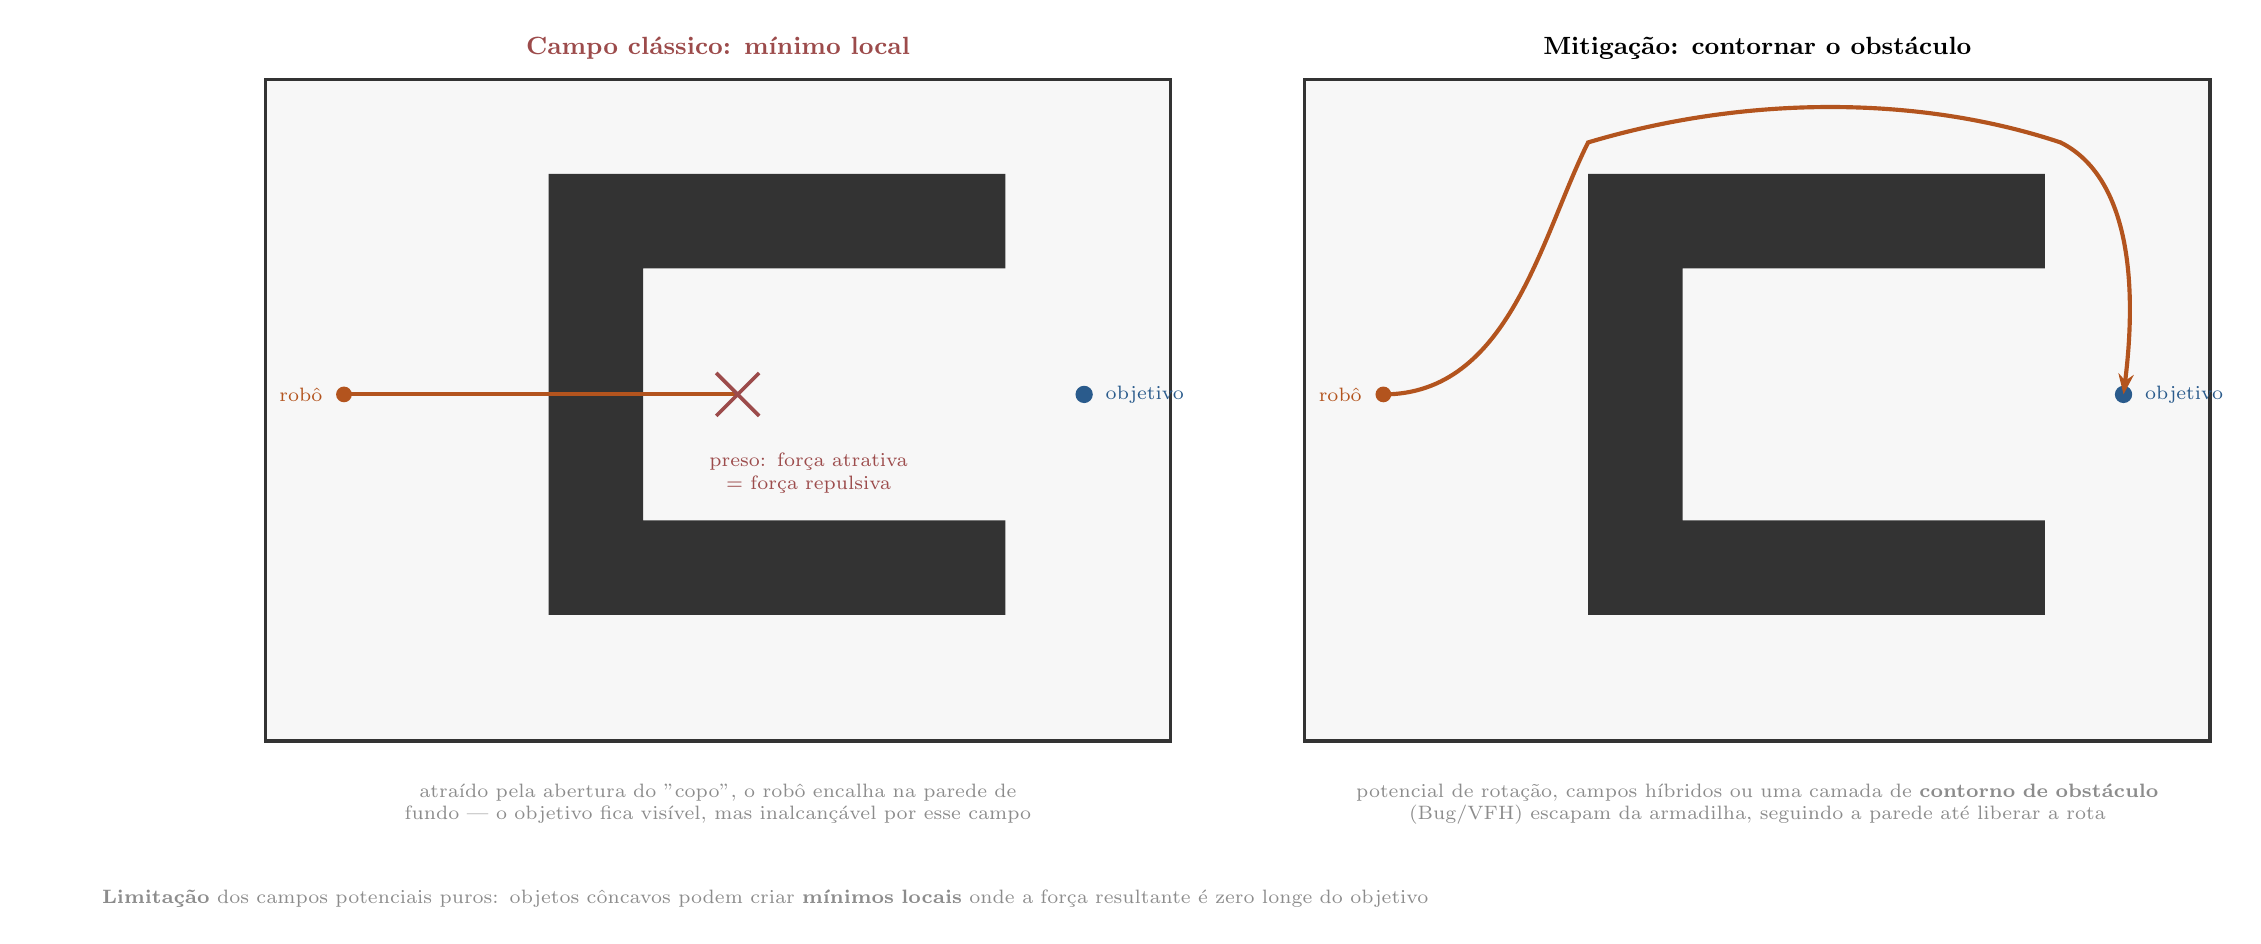
\begin{tikzpicture}[x=1cm,y=1cm]

  % Painel A: mínimo local (a armadilha do "copo")
  \begin{scope}[shift={(0,0)}]
    \draw[dbody, line width=1.2pt] (0,0) rectangle (11.5,8.4);
    \node[font=\bfseries\small, dred] at (5.75,8.8) {Campo clássico: mínimo local};

    \fill[black!80] (3.6,1.6) -- (3.6,7.2) -- (9.4,7.2) -- (9.4,6.0) -- (4.8,6.0)
                    -- (4.8,2.8) -- (9.4,2.8) -- (9.4,1.6) -- cycle;

    \fill[dblue] (10.4,4.4) circle (0.11);
    \node[dblue, font=\scriptsize, anchor=west] at (10.55,4.4) {objetivo};
    \fill[dorange] (1.0,4.4) circle (0.1);
    \node[dorange, font=\scriptsize, anchor=east] at (0.85,4.4) {robô};

    \draw[dcurveb, line width=1.5pt] (1.0,4.4) -- (6.0,4.4);
    \node[draw=dred, line width=1.3pt, cross out, minimum size=5mm, inner sep=0pt] at (6.0,4.4) {};
    \node[dred, font=\scriptsize, align=center, text width=3.2cm] at (6.9,3.4) {preso: força atrativa = força repulsiva};

    \node[dsub, font=\scriptsize, align=center, text width=10.8cm] at (5.75,-0.8)
       {atraído pela abertura do "copo", o robô encalha na parede de fundo --- o objetivo fica visível, mas inalcançável por esse campo};
  \end{scope}

  % Painel B: mitigação (contorno / potencial estendido)
  \begin{scope}[shift={(13.2,0)}]
    \draw[dbody, line width=1.2pt] (0,0) rectangle (11.5,8.4);
    \node[font=\bfseries\small] at (5.75,8.8) {Mitigação: contornar o obstáculo};

    \fill[black!80] (3.6,1.6) -- (3.6,7.2) -- (9.4,7.2) -- (9.4,6.0) -- (4.8,6.0)
                    -- (4.8,2.8) -- (9.4,2.8) -- (9.4,1.6) -- cycle;

    \fill[dblue] (10.4,4.4) circle (0.11);
    \node[dblue, font=\scriptsize, anchor=west] at (10.55,4.4) {objetivo};
    \fill[dorange] (1.0,4.4) circle (0.1);
    \node[dorange, font=\scriptsize, anchor=east] at (0.85,4.4) {robô};

    \draw[dcurveb, line width=1.5pt, -{Stealth[length=2.6mm]}]
      (1.0,4.4) .. controls (2.6,4.4) and (3.0,6.4) .. (3.6,7.6)
      .. controls (5.6,8.2) and (7.8,8.2) .. (9.6,7.6)
      .. controls (10.4,7.2) and (10.6,6.0) .. (10.4,4.4);

    \node[dsub, font=\scriptsize, align=center, text width=10.8cm] at (5.75,-0.8)
       {potencial de rotação, campos híbridos ou uma camada de \textbf{contorno de obstáculo} (Bug/VFH) escapam da armadilha, seguindo a parede até liberar a rota};
  \end{scope}

  \node[dsub, font=\scriptsize, align=center, text width=18.5cm] at (6.35,-2.0)
     {\textbf{Limitação} dos campos potenciais puros: objetos côncavos podem criar \textbf{mínimos locais} onde a força resultante é zero longe do objetivo};

\end{tikzpicture}
\end{document}
